% Created by tikzDevice version 0.12.3.1 on 2022-09-20 16:19:13
% !TEX encoding = UTF-8 Unicode
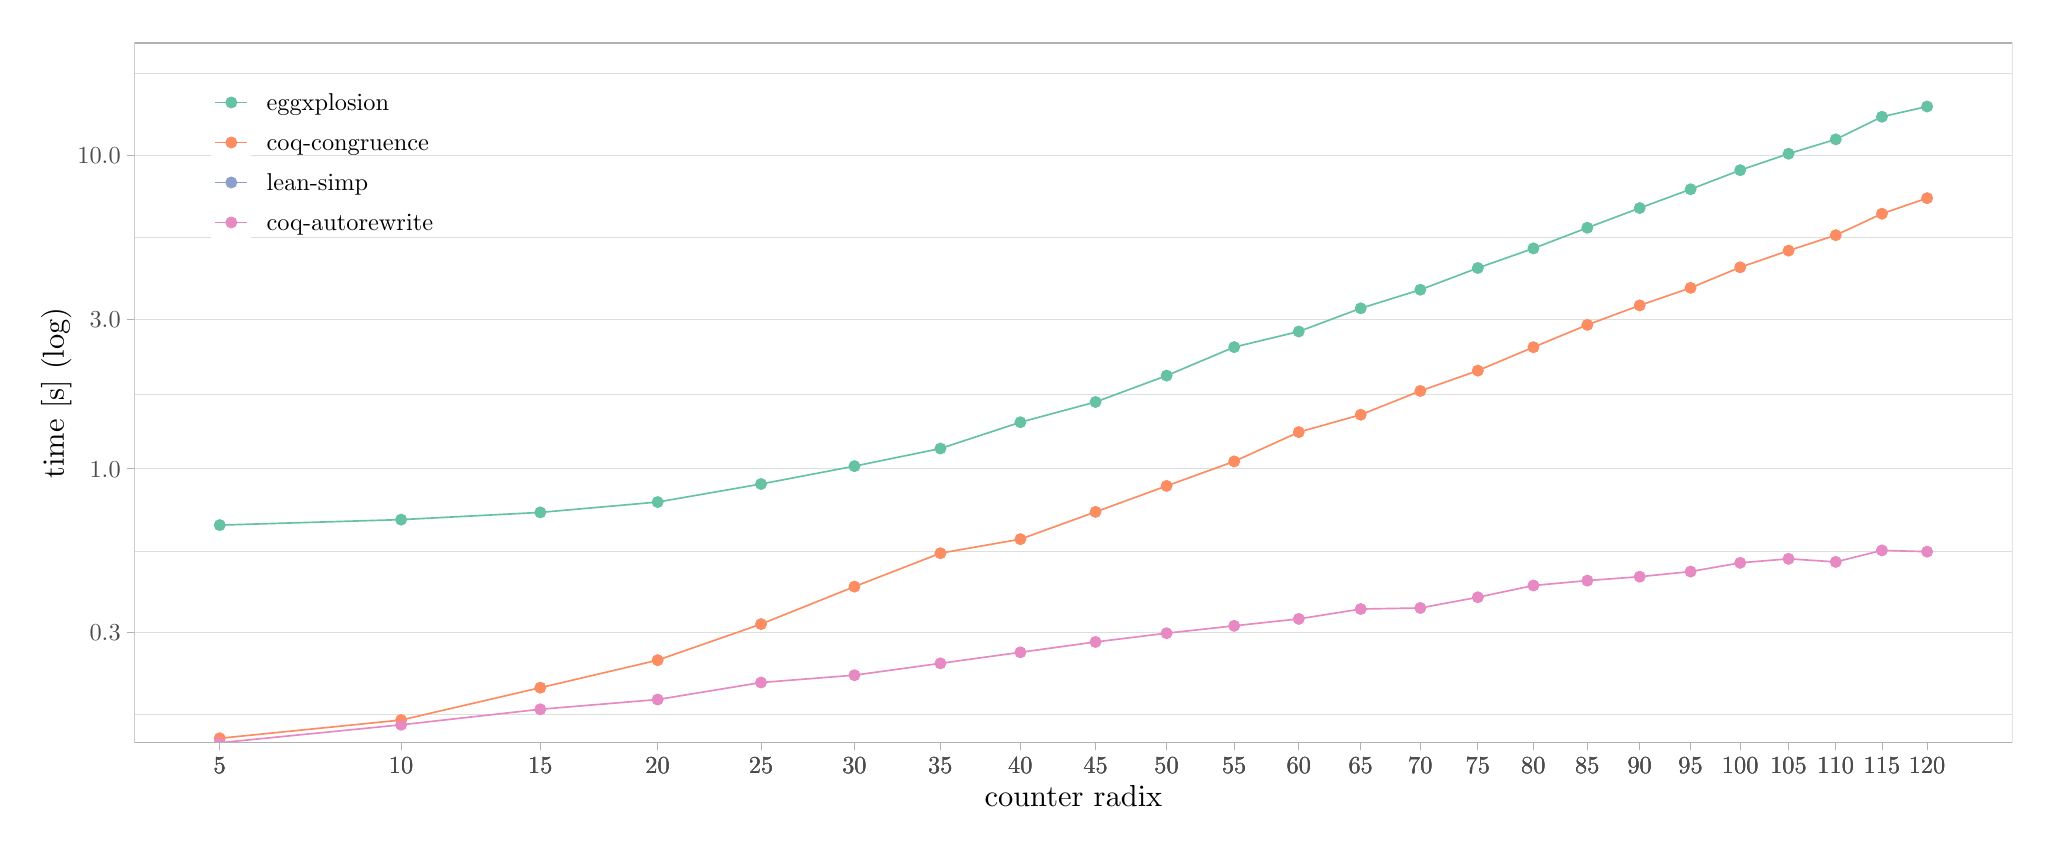
\begin{tikzpicture}[x=1pt,y=1pt]
\definecolor{fillColor}{RGB}{255,255,255}
\path[use as bounding box,fill=fillColor,fill opacity=0.00] (0,0) rectangle (722.70,289.08);
\begin{scope}
\path[clip] (  0.00,  0.00) rectangle (722.70,289.08);
\definecolor{drawColor}{RGB}{255,255,255}
\definecolor{fillColor}{RGB}{255,255,255}

\path[draw=drawColor,line width= 0.6pt,line join=round,line cap=round,fill=fillColor] (  0.00,  0.00) rectangle (722.70,289.08);
\end{scope}
\begin{scope}
\path[clip] ( 38.56, 30.69) rectangle (717.20,283.58);
\definecolor{fillColor}{RGB}{255,255,255}

\path[fill=fillColor] ( 38.56, 30.69) rectangle (717.20,283.58);
\definecolor{drawColor}{gray}{0.87}

\path[draw=drawColor,line width= 0.1pt,line join=round] ( 38.56, 40.88) --
	(717.20, 40.88);

\path[draw=drawColor,line width= 0.1pt,line join=round] ( 38.56,100.10) --
	(717.20,100.10);

\path[draw=drawColor,line width= 0.1pt,line join=round] ( 38.56,156.74) --
	(717.20,156.74);

\path[draw=drawColor,line width= 0.1pt,line join=round] ( 38.56,213.37) --
	(717.20,213.37);

\path[draw=drawColor,line width= 0.1pt,line join=round] ( 38.56,272.60) --
	(717.20,272.60);

\path[draw=drawColor,line width= 0.3pt,line join=round] ( 38.56, 70.49) --
	(717.20, 70.49);

\path[draw=drawColor,line width= 0.3pt,line join=round] ( 38.56,129.72) --
	(717.20,129.72);

\path[draw=drawColor,line width= 0.3pt,line join=round] ( 38.56,183.76) --
	(717.20,183.76);

\path[draw=drawColor,line width= 0.3pt,line join=round] ( 38.56,242.99) --
	(717.20,242.99);
\definecolor{drawColor}{RGB}{102,194,165}
\definecolor{fillColor}{RGB}{102,194,165}

\path[draw=drawColor,line width= 0.4pt,line join=round,line cap=round,fill=fillColor] ( 69.40,109.33) circle (  1.96);
\definecolor{drawColor}{RGB}{252,141,98}
\definecolor{fillColor}{RGB}{252,141,98}

\path[draw=drawColor,line width= 0.4pt,line join=round,line cap=round,fill=fillColor] ( 69.40, 32.30) circle (  1.96);
\definecolor{drawColor}{RGB}{231,138,195}
\definecolor{fillColor}{RGB}{231,138,195}

\path[draw=drawColor,line width= 0.4pt,line join=round,line cap=round,fill=fillColor] ( 69.40, 30.69) circle (  1.96);
\definecolor{drawColor}{RGB}{102,194,165}
\definecolor{fillColor}{RGB}{102,194,165}

\path[draw=drawColor,line width= 0.4pt,line join=round,line cap=round,fill=fillColor] (134.95,111.31) circle (  1.96);
\definecolor{drawColor}{RGB}{252,141,98}
\definecolor{fillColor}{RGB}{252,141,98}

\path[draw=drawColor,line width= 0.4pt,line join=round,line cap=round,fill=fillColor] (134.95, 38.89) circle (  1.96);
\definecolor{drawColor}{RGB}{231,138,195}
\definecolor{fillColor}{RGB}{231,138,195}

\path[draw=drawColor,line width= 0.4pt,line join=round,line cap=round,fill=fillColor] (134.95, 37.17) circle (  1.96);
\definecolor{drawColor}{RGB}{102,194,165}
\definecolor{fillColor}{RGB}{102,194,165}

\path[draw=drawColor,line width= 0.4pt,line join=round,line cap=round,fill=fillColor] (185.24,113.92) circle (  1.96);
\definecolor{drawColor}{RGB}{252,141,98}
\definecolor{fillColor}{RGB}{252,141,98}

\path[draw=drawColor,line width= 0.4pt,line join=round,line cap=round,fill=fillColor] (185.24, 50.58) circle (  1.96);
\definecolor{drawColor}{RGB}{231,138,195}
\definecolor{fillColor}{RGB}{231,138,195}

\path[draw=drawColor,line width= 0.4pt,line join=round,line cap=round,fill=fillColor] (185.24, 42.79) circle (  1.96);
\definecolor{drawColor}{RGB}{102,194,165}
\definecolor{fillColor}{RGB}{102,194,165}

\path[draw=drawColor,line width= 0.4pt,line join=round,line cap=round,fill=fillColor] (227.64,117.66) circle (  1.96);
\definecolor{drawColor}{RGB}{252,141,98}
\definecolor{fillColor}{RGB}{252,141,98}

\path[draw=drawColor,line width= 0.4pt,line join=round,line cap=round,fill=fillColor] (227.64, 60.53) circle (  1.96);
\definecolor{drawColor}{RGB}{231,138,195}
\definecolor{fillColor}{RGB}{231,138,195}

\path[draw=drawColor,line width= 0.4pt,line join=round,line cap=round,fill=fillColor] (227.64, 46.30) circle (  1.96);
\definecolor{drawColor}{RGB}{102,194,165}
\definecolor{fillColor}{RGB}{102,194,165}

\path[draw=drawColor,line width= 0.4pt,line join=round,line cap=round,fill=fillColor] (264.99,124.18) circle (  1.96);
\definecolor{drawColor}{RGB}{252,141,98}
\definecolor{fillColor}{RGB}{252,141,98}

\path[draw=drawColor,line width= 0.4pt,line join=round,line cap=round,fill=fillColor] (264.99, 73.56) circle (  1.96);
\definecolor{drawColor}{RGB}{231,138,195}
\definecolor{fillColor}{RGB}{231,138,195}

\path[draw=drawColor,line width= 0.4pt,line join=round,line cap=round,fill=fillColor] (264.99, 52.45) circle (  1.96);
\definecolor{drawColor}{RGB}{102,194,165}
\definecolor{fillColor}{RGB}{102,194,165}

\path[draw=drawColor,line width= 0.4pt,line join=round,line cap=round,fill=fillColor] (298.76,130.63) circle (  1.96);
\definecolor{drawColor}{RGB}{252,141,98}
\definecolor{fillColor}{RGB}{252,141,98}

\path[draw=drawColor,line width= 0.4pt,line join=round,line cap=round,fill=fillColor] (298.76, 87.10) circle (  1.96);
\definecolor{drawColor}{RGB}{231,138,195}
\definecolor{fillColor}{RGB}{231,138,195}

\path[draw=drawColor,line width= 0.4pt,line join=round,line cap=round,fill=fillColor] (298.76, 55.10) circle (  1.96);
\definecolor{drawColor}{RGB}{102,194,165}
\definecolor{fillColor}{RGB}{102,194,165}

\path[draw=drawColor,line width= 0.4pt,line join=round,line cap=round,fill=fillColor] (329.82,137.00) circle (  1.96);
\definecolor{drawColor}{RGB}{252,141,98}
\definecolor{fillColor}{RGB}{252,141,98}

\path[draw=drawColor,line width= 0.4pt,line join=round,line cap=round,fill=fillColor] (329.82, 99.18) circle (  1.96);
\definecolor{drawColor}{RGB}{231,138,195}
\definecolor{fillColor}{RGB}{231,138,195}

\path[draw=drawColor,line width= 0.4pt,line join=round,line cap=round,fill=fillColor] (329.82, 59.38) circle (  1.96);
\definecolor{drawColor}{RGB}{102,194,165}
\definecolor{fillColor}{RGB}{102,194,165}

\path[draw=drawColor,line width= 0.4pt,line join=round,line cap=round,fill=fillColor] (358.72,146.51) circle (  1.96);
\definecolor{drawColor}{RGB}{252,141,98}
\definecolor{fillColor}{RGB}{252,141,98}

\path[draw=drawColor,line width= 0.4pt,line join=round,line cap=round,fill=fillColor] (358.72,104.25) circle (  1.96);
\definecolor{drawColor}{RGB}{231,138,195}
\definecolor{fillColor}{RGB}{231,138,195}

\path[draw=drawColor,line width= 0.4pt,line join=round,line cap=round,fill=fillColor] (358.72, 63.37) circle (  1.96);
\definecolor{drawColor}{RGB}{102,194,165}
\definecolor{fillColor}{RGB}{102,194,165}

\path[draw=drawColor,line width= 0.4pt,line join=round,line cap=round,fill=fillColor] (385.87,153.82) circle (  1.96);
\definecolor{drawColor}{RGB}{252,141,98}
\definecolor{fillColor}{RGB}{252,141,98}

\path[draw=drawColor,line width= 0.4pt,line join=round,line cap=round,fill=fillColor] (385.87,114.10) circle (  1.96);
\definecolor{drawColor}{RGB}{231,138,195}
\definecolor{fillColor}{RGB}{231,138,195}

\path[draw=drawColor,line width= 0.4pt,line join=round,line cap=round,fill=fillColor] (385.87, 67.11) circle (  1.96);
\definecolor{drawColor}{RGB}{102,194,165}
\definecolor{fillColor}{RGB}{102,194,165}

\path[draw=drawColor,line width= 0.4pt,line join=round,line cap=round,fill=fillColor] (411.55,163.34) circle (  1.96);
\definecolor{drawColor}{RGB}{252,141,98}
\definecolor{fillColor}{RGB}{252,141,98}

\path[draw=drawColor,line width= 0.4pt,line join=round,line cap=round,fill=fillColor] (411.55,123.49) circle (  1.96);
\definecolor{drawColor}{RGB}{231,138,195}
\definecolor{fillColor}{RGB}{231,138,195}

\path[draw=drawColor,line width= 0.4pt,line join=round,line cap=round,fill=fillColor] (411.55, 70.27) circle (  1.96);
\definecolor{drawColor}{RGB}{102,194,165}
\definecolor{fillColor}{RGB}{102,194,165}

\path[draw=drawColor,line width= 0.4pt,line join=round,line cap=round,fill=fillColor] (435.97,173.65) circle (  1.96);
\definecolor{drawColor}{RGB}{252,141,98}
\definecolor{fillColor}{RGB}{252,141,98}

\path[draw=drawColor,line width= 0.4pt,line join=round,line cap=round,fill=fillColor] (435.97,132.35) circle (  1.96);
\definecolor{drawColor}{RGB}{231,138,195}
\definecolor{fillColor}{RGB}{231,138,195}

\path[draw=drawColor,line width= 0.4pt,line join=round,line cap=round,fill=fillColor] (435.97, 72.94) circle (  1.96);
\definecolor{drawColor}{RGB}{102,194,165}
\definecolor{fillColor}{RGB}{102,194,165}

\path[draw=drawColor,line width= 0.4pt,line join=round,line cap=round,fill=fillColor] (459.31,179.28) circle (  1.96);
\definecolor{drawColor}{RGB}{252,141,98}
\definecolor{fillColor}{RGB}{252,141,98}

\path[draw=drawColor,line width= 0.4pt,line join=round,line cap=round,fill=fillColor] (459.31,142.93) circle (  1.96);
\definecolor{drawColor}{RGB}{231,138,195}
\definecolor{fillColor}{RGB}{231,138,195}

\path[draw=drawColor,line width= 0.4pt,line join=round,line cap=round,fill=fillColor] (459.31, 75.44) circle (  1.96);
\definecolor{drawColor}{RGB}{102,194,165}
\definecolor{fillColor}{RGB}{102,194,165}

\path[draw=drawColor,line width= 0.4pt,line join=round,line cap=round,fill=fillColor] (481.69,187.67) circle (  1.96);
\definecolor{drawColor}{RGB}{252,141,98}
\definecolor{fillColor}{RGB}{252,141,98}

\path[draw=drawColor,line width= 0.4pt,line join=round,line cap=round,fill=fillColor] (481.69,149.21) circle (  1.96);
\definecolor{drawColor}{RGB}{231,138,195}
\definecolor{fillColor}{RGB}{231,138,195}

\path[draw=drawColor,line width= 0.4pt,line join=round,line cap=round,fill=fillColor] (481.69, 79.00) circle (  1.96);
\definecolor{drawColor}{RGB}{102,194,165}
\definecolor{fillColor}{RGB}{102,194,165}

\path[draw=drawColor,line width= 0.4pt,line join=round,line cap=round,fill=fillColor] (503.23,194.38) circle (  1.96);
\definecolor{drawColor}{RGB}{252,141,98}
\definecolor{fillColor}{RGB}{252,141,98}

\path[draw=drawColor,line width= 0.4pt,line join=round,line cap=round,fill=fillColor] (503.23,157.81) circle (  1.96);
\definecolor{drawColor}{RGB}{231,138,195}
\definecolor{fillColor}{RGB}{231,138,195}

\path[draw=drawColor,line width= 0.4pt,line join=round,line cap=round,fill=fillColor] (503.23, 79.39) circle (  1.96);
\definecolor{drawColor}{RGB}{102,194,165}
\definecolor{fillColor}{RGB}{102,194,165}

\path[draw=drawColor,line width= 0.4pt,line join=round,line cap=round,fill=fillColor] (524.01,202.24) circle (  1.96);
\definecolor{drawColor}{RGB}{252,141,98}
\definecolor{fillColor}{RGB}{252,141,98}

\path[draw=drawColor,line width= 0.4pt,line join=round,line cap=round,fill=fillColor] (524.01,165.15) circle (  1.96);
\definecolor{drawColor}{RGB}{231,138,195}
\definecolor{fillColor}{RGB}{231,138,195}

\path[draw=drawColor,line width= 0.4pt,line join=round,line cap=round,fill=fillColor] (524.01, 83.26) circle (  1.96);
\definecolor{drawColor}{RGB}{102,194,165}
\definecolor{fillColor}{RGB}{102,194,165}

\path[draw=drawColor,line width= 0.4pt,line join=round,line cap=round,fill=fillColor] (544.10,209.32) circle (  1.96);
\definecolor{drawColor}{RGB}{252,141,98}
\definecolor{fillColor}{RGB}{252,141,98}

\path[draw=drawColor,line width= 0.4pt,line join=round,line cap=round,fill=fillColor] (544.10,173.62) circle (  1.96);
\definecolor{drawColor}{RGB}{231,138,195}
\definecolor{fillColor}{RGB}{231,138,195}

\path[draw=drawColor,line width= 0.4pt,line join=round,line cap=round,fill=fillColor] (544.10, 87.51) circle (  1.96);
\definecolor{drawColor}{RGB}{102,194,165}
\definecolor{fillColor}{RGB}{102,194,165}

\path[draw=drawColor,line width= 0.4pt,line join=round,line cap=round,fill=fillColor] (563.58,216.78) circle (  1.96);
\definecolor{drawColor}{RGB}{252,141,98}
\definecolor{fillColor}{RGB}{252,141,98}

\path[draw=drawColor,line width= 0.4pt,line join=round,line cap=round,fill=fillColor] (563.58,181.69) circle (  1.96);
\definecolor{drawColor}{RGB}{231,138,195}
\definecolor{fillColor}{RGB}{231,138,195}

\path[draw=drawColor,line width= 0.4pt,line join=round,line cap=round,fill=fillColor] (563.58, 89.28) circle (  1.96);
\definecolor{drawColor}{RGB}{102,194,165}
\definecolor{fillColor}{RGB}{102,194,165}

\path[draw=drawColor,line width= 0.4pt,line join=round,line cap=round,fill=fillColor] (582.50,223.89) circle (  1.96);
\definecolor{drawColor}{RGB}{252,141,98}
\definecolor{fillColor}{RGB}{252,141,98}

\path[draw=drawColor,line width= 0.4pt,line join=round,line cap=round,fill=fillColor] (582.50,188.72) circle (  1.96);
\definecolor{drawColor}{RGB}{231,138,195}
\definecolor{fillColor}{RGB}{231,138,195}

\path[draw=drawColor,line width= 0.4pt,line join=round,line cap=round,fill=fillColor] (582.50, 90.69) circle (  1.96);
\definecolor{drawColor}{RGB}{102,194,165}
\definecolor{fillColor}{RGB}{102,194,165}

\path[draw=drawColor,line width= 0.4pt,line join=round,line cap=round,fill=fillColor] (600.89,230.69) circle (  1.96);
\definecolor{drawColor}{RGB}{252,141,98}
\definecolor{fillColor}{RGB}{252,141,98}

\path[draw=drawColor,line width= 0.4pt,line join=round,line cap=round,fill=fillColor] (600.89,195.06) circle (  1.96);
\definecolor{drawColor}{RGB}{231,138,195}
\definecolor{fillColor}{RGB}{231,138,195}

\path[draw=drawColor,line width= 0.4pt,line join=round,line cap=round,fill=fillColor] (600.89, 92.54) circle (  1.96);
\definecolor{drawColor}{RGB}{102,194,165}
\definecolor{fillColor}{RGB}{102,194,165}

\path[draw=drawColor,line width= 0.4pt,line join=round,line cap=round,fill=fillColor] (618.81,237.58) circle (  1.96);
\definecolor{drawColor}{RGB}{252,141,98}
\definecolor{fillColor}{RGB}{252,141,98}

\path[draw=drawColor,line width= 0.4pt,line join=round,line cap=round,fill=fillColor] (618.81,202.49) circle (  1.96);
\definecolor{drawColor}{RGB}{231,138,195}
\definecolor{fillColor}{RGB}{231,138,195}

\path[draw=drawColor,line width= 0.4pt,line join=round,line cap=round,fill=fillColor] (618.81, 95.70) circle (  1.96);
\definecolor{drawColor}{RGB}{102,194,165}
\definecolor{fillColor}{RGB}{102,194,165}

\path[draw=drawColor,line width= 0.4pt,line join=round,line cap=round,fill=fillColor] (636.29,243.53) circle (  1.96);
\definecolor{drawColor}{RGB}{252,141,98}
\definecolor{fillColor}{RGB}{252,141,98}

\path[draw=drawColor,line width= 0.4pt,line join=round,line cap=round,fill=fillColor] (636.29,208.51) circle (  1.96);
\definecolor{drawColor}{RGB}{231,138,195}
\definecolor{fillColor}{RGB}{231,138,195}

\path[draw=drawColor,line width= 0.4pt,line join=round,line cap=round,fill=fillColor] (636.29, 97.15) circle (  1.96);
\definecolor{drawColor}{RGB}{102,194,165}
\definecolor{fillColor}{RGB}{102,194,165}

\path[draw=drawColor,line width= 0.4pt,line join=round,line cap=round,fill=fillColor] (653.35,248.72) circle (  1.96);
\definecolor{drawColor}{RGB}{252,141,98}
\definecolor{fillColor}{RGB}{252,141,98}

\path[draw=drawColor,line width= 0.4pt,line join=round,line cap=round,fill=fillColor] (653.35,214.10) circle (  1.96);
\definecolor{drawColor}{RGB}{231,138,195}
\definecolor{fillColor}{RGB}{231,138,195}

\path[draw=drawColor,line width= 0.4pt,line join=round,line cap=round,fill=fillColor] (653.35, 96.03) circle (  1.96);
\definecolor{drawColor}{RGB}{102,194,165}
\definecolor{fillColor}{RGB}{102,194,165}

\path[draw=drawColor,line width= 0.4pt,line join=round,line cap=round,fill=fillColor] (670.03,256.88) circle (  1.96);
\definecolor{drawColor}{RGB}{252,141,98}
\definecolor{fillColor}{RGB}{252,141,98}

\path[draw=drawColor,line width= 0.4pt,line join=round,line cap=round,fill=fillColor] (670.03,221.85) circle (  1.96);
\definecolor{drawColor}{RGB}{231,138,195}
\definecolor{fillColor}{RGB}{231,138,195}

\path[draw=drawColor,line width= 0.4pt,line join=round,line cap=round,fill=fillColor] (670.03,100.19) circle (  1.96);
\definecolor{drawColor}{RGB}{102,194,165}
\definecolor{fillColor}{RGB}{102,194,165}

\path[draw=drawColor,line width= 0.4pt,line join=round,line cap=round,fill=fillColor] (686.35,260.59) circle (  1.96);
\definecolor{drawColor}{RGB}{252,141,98}
\definecolor{fillColor}{RGB}{252,141,98}

\path[draw=drawColor,line width= 0.4pt,line join=round,line cap=round,fill=fillColor] (686.35,227.47) circle (  1.96);
\definecolor{drawColor}{RGB}{231,138,195}
\definecolor{fillColor}{RGB}{231,138,195}

\path[draw=drawColor,line width= 0.4pt,line join=round,line cap=round,fill=fillColor] (686.35, 99.73) circle (  1.96);
\definecolor{drawColor}{RGB}{102,194,165}

\path[draw=drawColor,line width= 0.6pt,line join=round] ( 69.40,109.33) --
	(134.95,111.31) --
	(185.24,113.92) --
	(227.64,117.66) --
	(264.99,124.18) --
	(298.76,130.63) --
	(329.82,137.00) --
	(358.72,146.51) --
	(385.87,153.82) --
	(411.55,163.34) --
	(435.97,173.65) --
	(459.31,179.28) --
	(481.69,187.67) --
	(503.23,194.38) --
	(524.01,202.24) --
	(544.10,209.32) --
	(563.58,216.78) --
	(582.50,223.89) --
	(600.89,230.69) --
	(618.81,237.58) --
	(636.29,243.53) --
	(653.35,248.72) --
	(670.03,256.88) --
	(686.35,260.59);
\definecolor{drawColor}{RGB}{252,141,98}

\path[draw=drawColor,line width= 0.6pt,line join=round] ( 69.40, 32.30) --
	(134.95, 38.89) --
	(185.24, 50.58) --
	(227.64, 60.53) --
	(264.99, 73.56) --
	(298.76, 87.10) --
	(329.82, 99.18) --
	(358.72,104.25) --
	(385.87,114.10) --
	(411.55,123.49) --
	(435.97,132.35) --
	(459.31,142.93) --
	(481.69,149.21) --
	(503.23,157.81) --
	(524.01,165.15) --
	(544.10,173.62) --
	(563.58,181.69) --
	(582.50,188.72) --
	(600.89,195.06) --
	(618.81,202.49) --
	(636.29,208.51) --
	(653.35,214.10) --
	(670.03,221.85) --
	(686.35,227.47);
\definecolor{drawColor}{RGB}{231,138,195}

\path[draw=drawColor,line width= 0.6pt,line join=round] ( 69.40, 30.69) --
	(134.95, 37.17) --
	(185.24, 42.79) --
	(227.64, 46.30) --
	(264.99, 52.45) --
	(298.76, 55.10) --
	(329.82, 59.38) --
	(358.72, 63.37) --
	(385.87, 67.11) --
	(411.55, 70.27) --
	(435.97, 72.94) --
	(459.31, 75.44) --
	(481.69, 79.00) --
	(503.23, 79.39) --
	(524.01, 83.26) --
	(544.10, 87.51) --
	(563.58, 89.28) --
	(582.50, 90.69) --
	(600.89, 92.54) --
	(618.81, 95.70) --
	(636.29, 97.15) --
	(653.35, 96.03) --
	(670.03,100.19) --
	(686.35, 99.73);
\definecolor{drawColor}{gray}{0.70}

\path[draw=drawColor,line width= 0.6pt,line join=round,line cap=round] ( 38.56, 30.69) rectangle (717.20,283.58);
\end{scope}
\begin{scope}
\path[clip] (  0.00,  0.00) rectangle (722.70,289.08);
\definecolor{drawColor}{gray}{0.30}

\node[text=drawColor,anchor=base east,inner sep=0pt, outer sep=0pt, scale=  0.88] at ( 33.61, 67.46) {0.3};

\node[text=drawColor,anchor=base east,inner sep=0pt, outer sep=0pt, scale=  0.88] at ( 33.61,126.69) {1.0};

\node[text=drawColor,anchor=base east,inner sep=0pt, outer sep=0pt, scale=  0.88] at ( 33.61,180.73) {3.0};

\node[text=drawColor,anchor=base east,inner sep=0pt, outer sep=0pt, scale=  0.88] at ( 33.61,239.95) {10.0};
\end{scope}
\begin{scope}
\path[clip] (  0.00,  0.00) rectangle (722.70,289.08);
\definecolor{drawColor}{gray}{0.70}

\path[draw=drawColor,line width= 0.3pt,line join=round] ( 35.81, 70.49) --
	( 38.56, 70.49);

\path[draw=drawColor,line width= 0.3pt,line join=round] ( 35.81,129.72) --
	( 38.56,129.72);

\path[draw=drawColor,line width= 0.3pt,line join=round] ( 35.81,183.76) --
	( 38.56,183.76);

\path[draw=drawColor,line width= 0.3pt,line join=round] ( 35.81,242.99) --
	( 38.56,242.99);
\end{scope}
\begin{scope}
\path[clip] (  0.00,  0.00) rectangle (722.70,289.08);
\definecolor{drawColor}{gray}{0.70}

\path[draw=drawColor,line width= 0.3pt,line join=round] ( 69.40, 27.94) --
	( 69.40, 30.69);

\path[draw=drawColor,line width= 0.3pt,line join=round] ( 69.40, 27.94) --
	( 69.40, 30.69);

\path[draw=drawColor,line width= 0.3pt,line join=round] ( 69.40, 27.94) --
	( 69.40, 30.69);

\path[draw=drawColor,line width= 0.3pt,line join=round] ( 69.40, 27.94) --
	( 69.40, 30.69);

\path[draw=drawColor,line width= 0.3pt,line join=round] (134.95, 27.94) --
	(134.95, 30.69);

\path[draw=drawColor,line width= 0.3pt,line join=round] (134.95, 27.94) --
	(134.95, 30.69);

\path[draw=drawColor,line width= 0.3pt,line join=round] (134.95, 27.94) --
	(134.95, 30.69);

\path[draw=drawColor,line width= 0.3pt,line join=round] (185.24, 27.94) --
	(185.24, 30.69);

\path[draw=drawColor,line width= 0.3pt,line join=round] (185.24, 27.94) --
	(185.24, 30.69);

\path[draw=drawColor,line width= 0.3pt,line join=round] (185.24, 27.94) --
	(185.24, 30.69);

\path[draw=drawColor,line width= 0.3pt,line join=round] (227.64, 27.94) --
	(227.64, 30.69);

\path[draw=drawColor,line width= 0.3pt,line join=round] (227.64, 27.94) --
	(227.64, 30.69);

\path[draw=drawColor,line width= 0.3pt,line join=round] (227.64, 27.94) --
	(227.64, 30.69);

\path[draw=drawColor,line width= 0.3pt,line join=round] (264.99, 27.94) --
	(264.99, 30.69);

\path[draw=drawColor,line width= 0.3pt,line join=round] (264.99, 27.94) --
	(264.99, 30.69);

\path[draw=drawColor,line width= 0.3pt,line join=round] (264.99, 27.94) --
	(264.99, 30.69);

\path[draw=drawColor,line width= 0.3pt,line join=round] (298.76, 27.94) --
	(298.76, 30.69);

\path[draw=drawColor,line width= 0.3pt,line join=round] (298.76, 27.94) --
	(298.76, 30.69);

\path[draw=drawColor,line width= 0.3pt,line join=round] (298.76, 27.94) --
	(298.76, 30.69);

\path[draw=drawColor,line width= 0.3pt,line join=round] (329.82, 27.94) --
	(329.82, 30.69);

\path[draw=drawColor,line width= 0.3pt,line join=round] (329.82, 27.94) --
	(329.82, 30.69);

\path[draw=drawColor,line width= 0.3pt,line join=round] (329.82, 27.94) --
	(329.82, 30.69);

\path[draw=drawColor,line width= 0.3pt,line join=round] (358.72, 27.94) --
	(358.72, 30.69);

\path[draw=drawColor,line width= 0.3pt,line join=round] (358.72, 27.94) --
	(358.72, 30.69);

\path[draw=drawColor,line width= 0.3pt,line join=round] (358.72, 27.94) --
	(358.72, 30.69);

\path[draw=drawColor,line width= 0.3pt,line join=round] (385.87, 27.94) --
	(385.87, 30.69);

\path[draw=drawColor,line width= 0.3pt,line join=round] (385.87, 27.94) --
	(385.87, 30.69);

\path[draw=drawColor,line width= 0.3pt,line join=round] (385.87, 27.94) --
	(385.87, 30.69);

\path[draw=drawColor,line width= 0.3pt,line join=round] (411.55, 27.94) --
	(411.55, 30.69);

\path[draw=drawColor,line width= 0.3pt,line join=round] (411.55, 27.94) --
	(411.55, 30.69);

\path[draw=drawColor,line width= 0.3pt,line join=round] (411.55, 27.94) --
	(411.55, 30.69);

\path[draw=drawColor,line width= 0.3pt,line join=round] (435.97, 27.94) --
	(435.97, 30.69);

\path[draw=drawColor,line width= 0.3pt,line join=round] (435.97, 27.94) --
	(435.97, 30.69);

\path[draw=drawColor,line width= 0.3pt,line join=round] (435.97, 27.94) --
	(435.97, 30.69);

\path[draw=drawColor,line width= 0.3pt,line join=round] (459.31, 27.94) --
	(459.31, 30.69);

\path[draw=drawColor,line width= 0.3pt,line join=round] (459.31, 27.94) --
	(459.31, 30.69);

\path[draw=drawColor,line width= 0.3pt,line join=round] (459.31, 27.94) --
	(459.31, 30.69);

\path[draw=drawColor,line width= 0.3pt,line join=round] (481.69, 27.94) --
	(481.69, 30.69);

\path[draw=drawColor,line width= 0.3pt,line join=round] (481.69, 27.94) --
	(481.69, 30.69);

\path[draw=drawColor,line width= 0.3pt,line join=round] (481.69, 27.94) --
	(481.69, 30.69);

\path[draw=drawColor,line width= 0.3pt,line join=round] (503.23, 27.94) --
	(503.23, 30.69);

\path[draw=drawColor,line width= 0.3pt,line join=round] (503.23, 27.94) --
	(503.23, 30.69);

\path[draw=drawColor,line width= 0.3pt,line join=round] (503.23, 27.94) --
	(503.23, 30.69);

\path[draw=drawColor,line width= 0.3pt,line join=round] (524.01, 27.94) --
	(524.01, 30.69);

\path[draw=drawColor,line width= 0.3pt,line join=round] (524.01, 27.94) --
	(524.01, 30.69);

\path[draw=drawColor,line width= 0.3pt,line join=round] (524.01, 27.94) --
	(524.01, 30.69);

\path[draw=drawColor,line width= 0.3pt,line join=round] (544.10, 27.94) --
	(544.10, 30.69);

\path[draw=drawColor,line width= 0.3pt,line join=round] (544.10, 27.94) --
	(544.10, 30.69);

\path[draw=drawColor,line width= 0.3pt,line join=round] (544.10, 27.94) --
	(544.10, 30.69);

\path[draw=drawColor,line width= 0.3pt,line join=round] (563.58, 27.94) --
	(563.58, 30.69);

\path[draw=drawColor,line width= 0.3pt,line join=round] (563.58, 27.94) --
	(563.58, 30.69);

\path[draw=drawColor,line width= 0.3pt,line join=round] (563.58, 27.94) --
	(563.58, 30.69);

\path[draw=drawColor,line width= 0.3pt,line join=round] (582.50, 27.94) --
	(582.50, 30.69);

\path[draw=drawColor,line width= 0.3pt,line join=round] (582.50, 27.94) --
	(582.50, 30.69);

\path[draw=drawColor,line width= 0.3pt,line join=round] (582.50, 27.94) --
	(582.50, 30.69);

\path[draw=drawColor,line width= 0.3pt,line join=round] (600.89, 27.94) --
	(600.89, 30.69);

\path[draw=drawColor,line width= 0.3pt,line join=round] (600.89, 27.94) --
	(600.89, 30.69);

\path[draw=drawColor,line width= 0.3pt,line join=round] (600.89, 27.94) --
	(600.89, 30.69);

\path[draw=drawColor,line width= 0.3pt,line join=round] (618.81, 27.94) --
	(618.81, 30.69);

\path[draw=drawColor,line width= 0.3pt,line join=round] (618.81, 27.94) --
	(618.81, 30.69);

\path[draw=drawColor,line width= 0.3pt,line join=round] (618.81, 27.94) --
	(618.81, 30.69);

\path[draw=drawColor,line width= 0.3pt,line join=round] (636.29, 27.94) --
	(636.29, 30.69);

\path[draw=drawColor,line width= 0.3pt,line join=round] (636.29, 27.94) --
	(636.29, 30.69);

\path[draw=drawColor,line width= 0.3pt,line join=round] (636.29, 27.94) --
	(636.29, 30.69);

\path[draw=drawColor,line width= 0.3pt,line join=round] (653.35, 27.94) --
	(653.35, 30.69);

\path[draw=drawColor,line width= 0.3pt,line join=round] (653.35, 27.94) --
	(653.35, 30.69);

\path[draw=drawColor,line width= 0.3pt,line join=round] (653.35, 27.94) --
	(653.35, 30.69);

\path[draw=drawColor,line width= 0.3pt,line join=round] (670.03, 27.94) --
	(670.03, 30.69);

\path[draw=drawColor,line width= 0.3pt,line join=round] (670.03, 27.94) --
	(670.03, 30.69);

\path[draw=drawColor,line width= 0.3pt,line join=round] (670.03, 27.94) --
	(670.03, 30.69);

\path[draw=drawColor,line width= 0.3pt,line join=round] (686.35, 27.94) --
	(686.35, 30.69);

\path[draw=drawColor,line width= 0.3pt,line join=round] (686.35, 27.94) --
	(686.35, 30.69);

\path[draw=drawColor,line width= 0.3pt,line join=round] (686.35, 27.94) --
	(686.35, 30.69);
\end{scope}
\begin{scope}
\path[clip] (  0.00,  0.00) rectangle (722.70,289.08);
\definecolor{drawColor}{gray}{0.30}

\node[text=drawColor,anchor=base,inner sep=0pt, outer sep=0pt, scale=  0.88] at ( 69.40, 19.68) {5};

\node[text=drawColor,anchor=base,inner sep=0pt, outer sep=0pt, scale=  0.88] at ( 69.40, 19.68) {5};

\node[text=drawColor,anchor=base,inner sep=0pt, outer sep=0pt, scale=  0.88] at ( 69.40, 19.68) {5};

\node[text=drawColor,anchor=base,inner sep=0pt, outer sep=0pt, scale=  0.88] at ( 69.40, 19.68) {5};

\node[text=drawColor,anchor=base,inner sep=0pt, outer sep=0pt, scale=  0.88] at (134.95, 19.68) {10};

\node[text=drawColor,anchor=base,inner sep=0pt, outer sep=0pt, scale=  0.88] at (134.95, 19.68) {10};

\node[text=drawColor,anchor=base,inner sep=0pt, outer sep=0pt, scale=  0.88] at (134.95, 19.68) {10};

\node[text=drawColor,anchor=base,inner sep=0pt, outer sep=0pt, scale=  0.88] at (185.24, 19.68) {15};

\node[text=drawColor,anchor=base,inner sep=0pt, outer sep=0pt, scale=  0.88] at (185.24, 19.68) {15};

\node[text=drawColor,anchor=base,inner sep=0pt, outer sep=0pt, scale=  0.88] at (185.24, 19.68) {15};

\node[text=drawColor,anchor=base,inner sep=0pt, outer sep=0pt, scale=  0.88] at (227.64, 19.68) {20};

\node[text=drawColor,anchor=base,inner sep=0pt, outer sep=0pt, scale=  0.88] at (227.64, 19.68) {20};

\node[text=drawColor,anchor=base,inner sep=0pt, outer sep=0pt, scale=  0.88] at (227.64, 19.68) {20};

\node[text=drawColor,anchor=base,inner sep=0pt, outer sep=0pt, scale=  0.88] at (264.99, 19.68) {25};

\node[text=drawColor,anchor=base,inner sep=0pt, outer sep=0pt, scale=  0.88] at (264.99, 19.68) {25};

\node[text=drawColor,anchor=base,inner sep=0pt, outer sep=0pt, scale=  0.88] at (264.99, 19.68) {25};

\node[text=drawColor,anchor=base,inner sep=0pt, outer sep=0pt, scale=  0.88] at (298.76, 19.68) {30};

\node[text=drawColor,anchor=base,inner sep=0pt, outer sep=0pt, scale=  0.88] at (298.76, 19.68) {30};

\node[text=drawColor,anchor=base,inner sep=0pt, outer sep=0pt, scale=  0.88] at (298.76, 19.68) {30};

\node[text=drawColor,anchor=base,inner sep=0pt, outer sep=0pt, scale=  0.88] at (329.82, 19.68) {35};

\node[text=drawColor,anchor=base,inner sep=0pt, outer sep=0pt, scale=  0.88] at (329.82, 19.68) {35};

\node[text=drawColor,anchor=base,inner sep=0pt, outer sep=0pt, scale=  0.88] at (329.82, 19.68) {35};

\node[text=drawColor,anchor=base,inner sep=0pt, outer sep=0pt, scale=  0.88] at (358.72, 19.68) {40};

\node[text=drawColor,anchor=base,inner sep=0pt, outer sep=0pt, scale=  0.88] at (358.72, 19.68) {40};

\node[text=drawColor,anchor=base,inner sep=0pt, outer sep=0pt, scale=  0.88] at (358.72, 19.68) {40};

\node[text=drawColor,anchor=base,inner sep=0pt, outer sep=0pt, scale=  0.88] at (385.87, 19.68) {45};

\node[text=drawColor,anchor=base,inner sep=0pt, outer sep=0pt, scale=  0.88] at (385.87, 19.68) {45};

\node[text=drawColor,anchor=base,inner sep=0pt, outer sep=0pt, scale=  0.88] at (385.87, 19.68) {45};

\node[text=drawColor,anchor=base,inner sep=0pt, outer sep=0pt, scale=  0.88] at (411.55, 19.68) {50};

\node[text=drawColor,anchor=base,inner sep=0pt, outer sep=0pt, scale=  0.88] at (411.55, 19.68) {50};

\node[text=drawColor,anchor=base,inner sep=0pt, outer sep=0pt, scale=  0.88] at (411.55, 19.68) {50};

\node[text=drawColor,anchor=base,inner sep=0pt, outer sep=0pt, scale=  0.88] at (435.97, 19.68) {55};

\node[text=drawColor,anchor=base,inner sep=0pt, outer sep=0pt, scale=  0.88] at (435.97, 19.68) {55};

\node[text=drawColor,anchor=base,inner sep=0pt, outer sep=0pt, scale=  0.88] at (435.97, 19.68) {55};

\node[text=drawColor,anchor=base,inner sep=0pt, outer sep=0pt, scale=  0.88] at (459.31, 19.68) {60};

\node[text=drawColor,anchor=base,inner sep=0pt, outer sep=0pt, scale=  0.88] at (459.31, 19.68) {60};

\node[text=drawColor,anchor=base,inner sep=0pt, outer sep=0pt, scale=  0.88] at (459.31, 19.68) {60};

\node[text=drawColor,anchor=base,inner sep=0pt, outer sep=0pt, scale=  0.88] at (481.69, 19.68) {65};

\node[text=drawColor,anchor=base,inner sep=0pt, outer sep=0pt, scale=  0.88] at (481.69, 19.68) {65};

\node[text=drawColor,anchor=base,inner sep=0pt, outer sep=0pt, scale=  0.88] at (481.69, 19.68) {65};

\node[text=drawColor,anchor=base,inner sep=0pt, outer sep=0pt, scale=  0.88] at (503.23, 19.68) {70};

\node[text=drawColor,anchor=base,inner sep=0pt, outer sep=0pt, scale=  0.88] at (503.23, 19.68) {70};

\node[text=drawColor,anchor=base,inner sep=0pt, outer sep=0pt, scale=  0.88] at (503.23, 19.68) {70};

\node[text=drawColor,anchor=base,inner sep=0pt, outer sep=0pt, scale=  0.88] at (524.01, 19.68) {75};

\node[text=drawColor,anchor=base,inner sep=0pt, outer sep=0pt, scale=  0.88] at (524.01, 19.68) {75};

\node[text=drawColor,anchor=base,inner sep=0pt, outer sep=0pt, scale=  0.88] at (524.01, 19.68) {75};

\node[text=drawColor,anchor=base,inner sep=0pt, outer sep=0pt, scale=  0.88] at (544.10, 19.68) {80};

\node[text=drawColor,anchor=base,inner sep=0pt, outer sep=0pt, scale=  0.88] at (544.10, 19.68) {80};

\node[text=drawColor,anchor=base,inner sep=0pt, outer sep=0pt, scale=  0.88] at (544.10, 19.68) {80};

\node[text=drawColor,anchor=base,inner sep=0pt, outer sep=0pt, scale=  0.88] at (563.58, 19.68) {85};

\node[text=drawColor,anchor=base,inner sep=0pt, outer sep=0pt, scale=  0.88] at (563.58, 19.68) {85};

\node[text=drawColor,anchor=base,inner sep=0pt, outer sep=0pt, scale=  0.88] at (563.58, 19.68) {85};

\node[text=drawColor,anchor=base,inner sep=0pt, outer sep=0pt, scale=  0.88] at (582.50, 19.68) {90};

\node[text=drawColor,anchor=base,inner sep=0pt, outer sep=0pt, scale=  0.88] at (582.50, 19.68) {90};

\node[text=drawColor,anchor=base,inner sep=0pt, outer sep=0pt, scale=  0.88] at (582.50, 19.68) {90};

\node[text=drawColor,anchor=base,inner sep=0pt, outer sep=0pt, scale=  0.88] at (600.89, 19.68) {95};

\node[text=drawColor,anchor=base,inner sep=0pt, outer sep=0pt, scale=  0.88] at (600.89, 19.68) {95};

\node[text=drawColor,anchor=base,inner sep=0pt, outer sep=0pt, scale=  0.88] at (600.89, 19.68) {95};

\node[text=drawColor,anchor=base,inner sep=0pt, outer sep=0pt, scale=  0.88] at (618.81, 19.68) {100};

\node[text=drawColor,anchor=base,inner sep=0pt, outer sep=0pt, scale=  0.88] at (618.81, 19.68) {100};

\node[text=drawColor,anchor=base,inner sep=0pt, outer sep=0pt, scale=  0.88] at (618.81, 19.68) {100};

\node[text=drawColor,anchor=base,inner sep=0pt, outer sep=0pt, scale=  0.88] at (636.29, 19.68) {105};

\node[text=drawColor,anchor=base,inner sep=0pt, outer sep=0pt, scale=  0.88] at (636.29, 19.68) {105};

\node[text=drawColor,anchor=base,inner sep=0pt, outer sep=0pt, scale=  0.88] at (636.29, 19.68) {105};

\node[text=drawColor,anchor=base,inner sep=0pt, outer sep=0pt, scale=  0.88] at (653.35, 19.68) {110};

\node[text=drawColor,anchor=base,inner sep=0pt, outer sep=0pt, scale=  0.88] at (653.35, 19.68) {110};

\node[text=drawColor,anchor=base,inner sep=0pt, outer sep=0pt, scale=  0.88] at (653.35, 19.68) {110};

\node[text=drawColor,anchor=base,inner sep=0pt, outer sep=0pt, scale=  0.88] at (670.03, 19.68) {115};

\node[text=drawColor,anchor=base,inner sep=0pt, outer sep=0pt, scale=  0.88] at (670.03, 19.68) {115};

\node[text=drawColor,anchor=base,inner sep=0pt, outer sep=0pt, scale=  0.88] at (670.03, 19.68) {115};

\node[text=drawColor,anchor=base,inner sep=0pt, outer sep=0pt, scale=  0.88] at (686.35, 19.68) {120};

\node[text=drawColor,anchor=base,inner sep=0pt, outer sep=0pt, scale=  0.88] at (686.35, 19.68) {120};

\node[text=drawColor,anchor=base,inner sep=0pt, outer sep=0pt, scale=  0.88] at (686.35, 19.68) {120};
\end{scope}
\begin{scope}
\path[clip] (  0.00,  0.00) rectangle (722.70,289.08);
\definecolor{drawColor}{RGB}{0,0,0}

\node[text=drawColor,anchor=base,inner sep=0pt, outer sep=0pt, scale=  1.10] at (377.88,  7.64) {counter radix};
\end{scope}
\begin{scope}
\path[clip] (  0.00,  0.00) rectangle (722.70,289.08);
\definecolor{drawColor}{RGB}{0,0,0}

\node[text=drawColor,rotate= 90.00,anchor=base,inner sep=0pt, outer sep=0pt, scale=  1.10] at ( 13.08,157.13) {time [s] (log)};
\end{scope}
\begin{scope}
\path[clip] (  0.00,  0.00) rectangle (722.70,289.08);
\definecolor{fillColor}{RGB}{255,255,255}

\path[fill=fillColor] ( 66.36,254.82) rectangle ( 80.81,269.27);
\end{scope}
\begin{scope}
\path[clip] (  0.00,  0.00) rectangle (722.70,289.08);
\definecolor{drawColor}{RGB}{102,194,165}
\definecolor{fillColor}{RGB}{102,194,165}

\path[draw=drawColor,line width= 0.4pt,line join=round,line cap=round,fill=fillColor] ( 73.59,262.05) circle (  1.96);
\end{scope}
\begin{scope}
\path[clip] (  0.00,  0.00) rectangle (722.70,289.08);
\definecolor{drawColor}{RGB}{102,194,165}

\path[draw=drawColor,line width= 0.6pt,line join=round] ( 67.80,262.05) -- ( 79.37,262.05);
\end{scope}
\begin{scope}
\path[clip] (  0.00,  0.00) rectangle (722.70,289.08);
\definecolor{fillColor}{RGB}{255,255,255}

\path[fill=fillColor] ( 66.36,240.37) rectangle ( 80.81,254.82);
\end{scope}
\begin{scope}
\path[clip] (  0.00,  0.00) rectangle (722.70,289.08);
\definecolor{drawColor}{RGB}{252,141,98}
\definecolor{fillColor}{RGB}{252,141,98}

\path[draw=drawColor,line width= 0.4pt,line join=round,line cap=round,fill=fillColor] ( 73.59,247.59) circle (  1.96);
\end{scope}
\begin{scope}
\path[clip] (  0.00,  0.00) rectangle (722.70,289.08);
\definecolor{drawColor}{RGB}{252,141,98}

\path[draw=drawColor,line width= 0.6pt,line join=round] ( 67.80,247.59) -- ( 79.37,247.59);
\end{scope}
\begin{scope}
\path[clip] (  0.00,  0.00) rectangle (722.70,289.08);
\definecolor{fillColor}{RGB}{255,255,255}

\path[fill=fillColor] ( 66.36,225.91) rectangle ( 80.81,240.37);
\end{scope}
\begin{scope}
\path[clip] (  0.00,  0.00) rectangle (722.70,289.08);
\definecolor{drawColor}{RGB}{141,160,203}
\definecolor{fillColor}{RGB}{141,160,203}

\path[draw=drawColor,line width= 0.4pt,line join=round,line cap=round,fill=fillColor] ( 73.59,233.14) circle (  1.96);
\end{scope}
\begin{scope}
\path[clip] (  0.00,  0.00) rectangle (722.70,289.08);
\definecolor{drawColor}{RGB}{141,160,203}

\path[draw=drawColor,line width= 0.6pt,line join=round] ( 67.80,233.14) -- ( 79.37,233.14);
\end{scope}
\begin{scope}
\path[clip] (  0.00,  0.00) rectangle (722.70,289.08);
\definecolor{fillColor}{RGB}{255,255,255}

\path[fill=fillColor] ( 66.36,211.46) rectangle ( 80.81,225.91);
\end{scope}
\begin{scope}
\path[clip] (  0.00,  0.00) rectangle (722.70,289.08);
\definecolor{drawColor}{RGB}{231,138,195}
\definecolor{fillColor}{RGB}{231,138,195}

\path[draw=drawColor,line width= 0.4pt,line join=round,line cap=round,fill=fillColor] ( 73.59,218.69) circle (  1.96);
\end{scope}
\begin{scope}
\path[clip] (  0.00,  0.00) rectangle (722.70,289.08);
\definecolor{drawColor}{RGB}{231,138,195}

\path[draw=drawColor,line width= 0.6pt,line join=round] ( 67.80,218.69) -- ( 79.37,218.69);
\end{scope}
\begin{scope}
\path[clip] (  0.00,  0.00) rectangle (722.70,289.08);
\definecolor{drawColor}{RGB}{0,0,0}

\node[text=drawColor,anchor=base west,inner sep=0pt, outer sep=0pt, scale=  0.88] at ( 86.31,259.02) {eggxplosion};
\end{scope}
\begin{scope}
\path[clip] (  0.00,  0.00) rectangle (722.70,289.08);
\definecolor{drawColor}{RGB}{0,0,0}

\node[text=drawColor,anchor=base west,inner sep=0pt, outer sep=0pt, scale=  0.88] at ( 86.31,244.56) {coq-congruence};
\end{scope}
\begin{scope}
\path[clip] (  0.00,  0.00) rectangle (722.70,289.08);
\definecolor{drawColor}{RGB}{0,0,0}

\node[text=drawColor,anchor=base west,inner sep=0pt, outer sep=0pt, scale=  0.88] at ( 86.31,230.11) {lean-simp};
\end{scope}
\begin{scope}
\path[clip] (  0.00,  0.00) rectangle (722.70,289.08);
\definecolor{drawColor}{RGB}{0,0,0}

\node[text=drawColor,anchor=base west,inner sep=0pt, outer sep=0pt, scale=  0.88] at ( 86.31,215.66) {coq-autorewrite};
\end{scope}
\end{tikzpicture}
